\documentclass[a4j,12pt,landscape]{tarticle}
\pagestyle{empty}
\usepackage[dvipdfmx]{graphicx}
\usepackage[deluxe]{otf}
\usepackage{plext}
\setlength{\columnseprule}{0.8pt}

\begin{document}
\rmfamily\mcfamily
% タイトル
\vspace{3.5cm}
\textbf{\huge 縦書き\TeX サンプル}

\vspace{0.5cm}
\hspace{2.5cm}

% 名前 (\Large ○○○) ... ○には全角空白15個むりやり
\begin{center}
  \textbf{\large                武産 合氣}
\end{center}

\hspace{2.5cm}

% platex <filename>.tex
% dvipdfmx -p a4 -l <filename>.dvi
% ↑↑↑ A4用紙の一行は長すぎるため, PDF生成時にうまくいくように明示する.
% \usepackage{plext}で縦横操作が可能(以下、使い方は2つ目のURL参考に)

% 参考: http://www.fugenji.org/~thomas/texlive-guide/vertical.html
% これとか https://qiita.com/zr_tex8r/items/6f0b88c5838c42241457

% ここから本文
初段取得時に小論文を\TeX で書きたい人向け。めんどくさい人はオフィスツール、または、手書きで。小論文は原稿用紙(縦書き)を使用すると思う。\TeX のマクロである\LaTeX は基本横書きだが、縦書きも一応できる。\LaTeX で書くメリットはいくつかある。\par
\LaTeX は体裁の調整が面倒。逆に言えば、体裁さえできていればあとは文とか数式を書くだけなので、ワードのように書いてる最中に体裁をいちいち考える必要がない。(要は、この説明文を書き換えれば小論文が書けます) 文字サイズやフォントが勝手に変わったりもしないし、クラッシュしてデータが消える恐れも少ない。とまあ、メリットはこのくらいにして以下に説明を書く。\par
縦書きサンプル文。1,2,3とかの数字はそのまま横書きになる。一応以下のように、「\pbox<y>{14}」と書くこともできる。縦書きが基本の場合に横書きとなる。他にもいろいろ使い方があるのでソースのURLを参考にするとよい。\par
なお、このサンプルは\TeX Live2017の環境下で作成した。platexでの実行を前提としているため、それ以外の動作は保証できないのであしからず。dvipdfmxでのPDF作成時にそのまま実行すると文書がおかしくなる(図\ref{fig:one})ので、ソースのコンパイル方法を参考にしてほしい。\par
最後に、初段取得時は小論文を提出するのが普通なので、必ず書きましょう。% make by masuda.


\vspace{1cm}

\begin{figure}[htbp]
 \begin{center}
  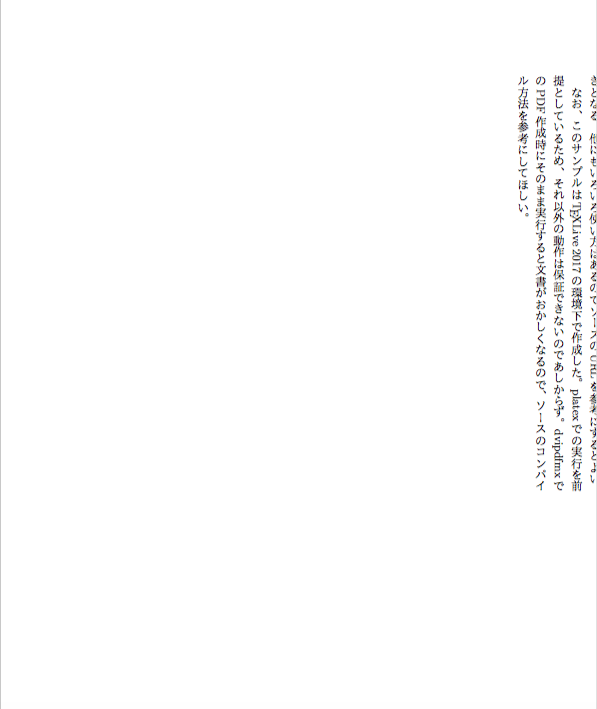
\includegraphics[width=5cm, height=9cm, angle=90]{err.png}
 \end{center}
 \caption{失敗例}
 \label{fig:one}
\end{figure}

\end{document}
